\documentclass{article}

\usepackage{amsmath} % 用于数学公式
\usepackage{graphicx} % 用于插入图片
\usepackage{lipsum} % 用于生成虚拟文本
\usepackage{ctex} % 导入 ctex 包以支持中文
\usepackage{titlesec} % 导入 titlesec 包以定制标题样式
\usepackage{fontspec} % 用于设置中文字体
\usepackage{amsfonts} 
\usepackage{amsmath} % 提供 \text 和 \tanh 命令
\usepackage{bm}      % 提供 \bm 命令用于粗体


\setmainfont{SimSun} % 设置中文字体,SimSun 为宋体的系统字体

\title{LinkPrediction实验}
\author{程智镝、陈凌}
\date{\today}

\begin{document}
\maketitle

\section*{作业任务}
\begin{itemize}
    \item 从代码(自己实现or复现)、数据集(直接获取或自己处理得到)两个角度权衡是否选择某个link prediction的工作。。
    \item 论文摘要abstract和introduction翻译
    \item 问题描述。
    \item 输入、输出、模型算法描述(附框架图;有多个的挑1个主要实现)
    \item 评价指标及其计算公式
    \item 对比方法及这些对比方法的引用论文出处
    \item 结果
    \item 打包提交code、运行配置说明(数据集太大的可以是开放链接,需描述)
\end{itemize}
\section*{实验难点:}
\begin{itemize}
    \item 论文为全英文描述,阅读难度提升
    \item 论文实验复现环境搭配
    \item 相关神经网络、机器学习、图论的知识暂且未知
\end{itemize}
\section*{实验准备工作}
\textbf{依赖下载:}
\begin{itemize}
\item cuda=11.3
\item pytorch=1.12.1
\item dgl-cuda11.3-0.9.1post
\item ogb=1.3.5
\item numpy=1.24.3
\item 数据集使用的是 ogbn- proteins dataset,实验使用的源码在\verb|https://github.com/houyili/gipa wide deep|
\end{itemize}
\textbf{服务器配置:}
\begin{figure}[htbp]
    \centering
    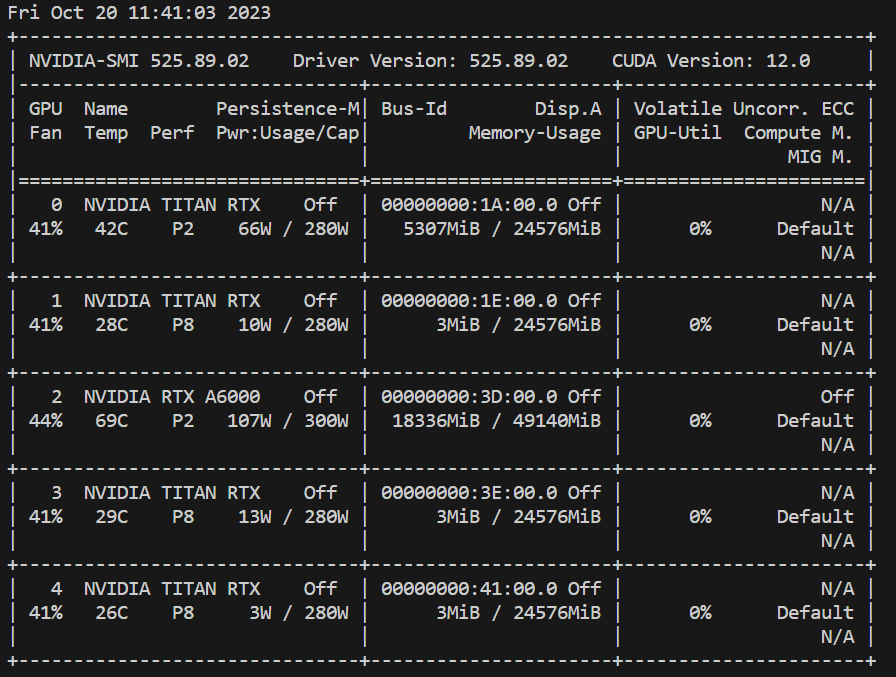
\includegraphics[width=9.5cm,height=8cm]{服务器配置.png}
\end{figure}
\section*{配置步骤}
\begin{enumerate}
\item 创建环境conda create -n gipa python=3.9
\item 用户文件下载GitHub代码:/data/zyk
\item python版本:3.9.18
\item 安装指定版本的 CUDA:conda install -c anaconda cudatoolkit=11.3
\item 下载dgl:conda install -c dglteam dgl-cuda11.3
\item numpy自带1.24.3
\item ogb下载:conda install ogb=1.3.5  这步下载了一个多小时……
\end{enumerate}
\section*{论文:GIPA: A General Information Propagation
Algorithm for Graph Learning}
\subsection*{abstract和introduction翻译}

\textbf{摘要:}图神经网络已经广泛应用于图结构数据计算,在节点类、链路预测和网络推荐等各种应用中显示出良好性能
现有工作主要集中在基于注意力对相邻节点进行加权聚合时的节点相关性,例如两个节点的密集向量的点积。这可能导致在进行信息传播时
要传播的节点中的冲突噪声。为了解决这个问题,我们提出了一种通用信息传播算法(GIPA),该算法利用了更细粒度的信息融合,
包括基于边缘特征的比特和特征相关性。具体地,逐位相关通过多层感知器(MLP)基于两个节点及其边缘的密集表示来计算逐元素注意力权重;
按特征的相关性基于用于特征选择的节点属性特征的一次热表示。我们在阿里巴巴集团的开放图基准蛋白数据集
和支付宝数据集上评估了GIPA的性能。结果表明GIPA在预测精度方面优于最先进的模型。例如,GIPA的平均ROC-AUC为0.8917±0.0007,优于
OGBN蛋白质排行榜上列出的所有现有方法。
关键词:图神经网络,细粒度信息融合,逐位和特征关注\\

\textbf{引言:}图表示学习通常旨在基于图拓扑(链接)信息为每个图节点学习信息嵌入。通常的,
节点的嵌入表示为低维特征向量,可用于促进下游应用。本文主要研究只有一类节点和一类边的齐次图。
目的是从图拓扑中学习节点表示。具体地,给定节点u,使用广度优先搜索、深度优先搜索或随机游动来识别一组相邻节点。
然后通过最大化u及其邻居的共现概率来学习u的嵌入。关于图嵌入的早期研究从图中捕获相邻信息的能力有限,
因为他们基于SkippGram等浅层学习模型。此外,在这些图嵌入方法中使用了转导学习,不能将其推广到训练图中不存在的新节点。\\
图神经网络是为了克服传统图嵌入模型的局限性而提出的。GNN(图神经网络)使用使用深度神经网络来句和来自相邻节点的特征信息,
并从而具有获得更好的聚合嵌入的潜力。GNN可以支持归纳学习,并在预测的过程中推断出看不见节点的类标签。
GNN的成功主要归功于领域信息的聚合。然而,GNN面临两个挑战:目标结点的那些相邻节点参与消息传递?以及每个相邻节点对聚合嵌入的贡献有多大?
对于前一个问题,对于大的稠密图或者幂律图,提出了邻域采样。
对于后者,邻居重要性估计用于在特征传播期间将不同的权重附加到不同的邻居节点。重要性抽样和注意力是两种流行的技术。
重要性采样是邻域采样的一种特殊情况,其中相邻节点的重要性权重是从结点上的分布中提取的。该分布可以从归一化拉普拉斯矩阵中导出,
也可以与GNN联合学习。利用这种分布,在每一步对邻居的自己进行采样,并用重要性权重进行聚合。与重要性抽样类似,注意力也将重要性权重赋予邻居。
然而,注意力不同于重要性抽样。注意力被表示为神经网络,并且总是作为GNN模型的一部分来学习。相反,重要性采样算法使用没有可训练参数的统计模型。\\
现有的注意力机制只考虑节点的相关性,忽略了传输噪声信息的抑制和边缘特征的信息。在现实世界的应用程序中,只有部分用户授权系统收集他们的配置文件。
该模型无法了解已配置文件的用户和我们一无所知的用户之间的节点相关性。因此,现有模型会传播噪声信息,导致节点表示不准确。
然而,两个经常相互转账的用户只进行了几次对话的用户具有不同的相关性。\\
为了解决上述问题,本文提出了一种新的图神经网络注意力模型,即广义信息传播模型(GIPA)我们设计了一个位相关模块和一个特征相关模块。具体而言,我们认为密集向量的每个维度表示节点的一个特征。因此,位相关模块在密集表示级别进行过滤。注意力权重的维度与密度向量相等。此外,我们将节点的每个属性特征表示为一个独热向量。特征相关模块通过输出具有相似维度和属性特征的注意力权重来执行特征选择。值得一提的是,为了使模型能够提取更好的注意力权重,度量节点之间相关性的边缘特征也包括在注意力计算中。最后,GIPA将稀疏嵌入和密集嵌入输入到深度神经网络的宽端和深端,分别用于学习特定任务。我们的贡献总结如下:

1) 我们设计了位相关模块和特征相关模块,以从元素级和特征级执行更精细的信息加权聚合,并利用了边缘信息。

2) 基于宽深度架构[6],我们使用密集特征表示和稀疏特征表示分别提取深层信息和保留浅层原始信息,为下游任务提供更全面的信息。

3) 在开放图基准(OGB)[11]蛋白质数据集(OGBN-proteins)上的实验证明,GIPA在OGBN-proteins排行榜上取得了更好的准确性,平均ROC-AUC为0.8917±0.0007,优于排行榜上列出的最先进方法。此外,GIPA已在亿级规模的支付宝工业数据集上进行了测试。
\section*{问题描述}


\section*{链路预测--Link Prediction}
\subsection*{图论前导知识}
假设有图 $G = (V, E, A)$,其中 $V$ 为图的节点集合,
$E$ 为图的边集合,而张量 $A \in \mathbb{R}^{n \times n \times d}$ 
包含了所有节点的属性(例如,用户资料)和边的属性(例如,交互作用的强度或类型)。对于每个节点 $v \in V$,它的属性(如果有的话)存储在对角组件 $A_{vv}$ 中,而非对角线组件 $A_{uv}$ 则可以包含边 $(u, v)$ 的属性,如果 $(u, v) \in E$;否则 $A_{uv} = 0$。
\subsection*{链路预测问题}
在链路预测中的目标是根据观察到的张量 $A$ 推断目标节点对之间是否存在边。学习问题是找到一个似然(或评分)函数 $f$,它为每对目标节点$(u, v) \notin E$ 分配交互似然性(分数) $\hat{A}_{uv}$,这些节点之间的关系未被观察到。较大的 $\hat{A}_{uv}$ 表示 $(u, v)$ 形成链接或缺失链接的可能性较高。函数 $f$ 可以表示为 $\hat{A}_{uv} = f(u, v, A|\Theta)$,其中 $\Theta$ 表示模型参数。
\section*{目的}
GIPA(通用信息传播算法)的目标是通过在传播过程中合并节点和边缘嵌入来改进图学习。
它旨在捕获图数据中的细粒度信息传播和噪声过滤。GIPA通过按位和特征相关模块的组合来实现这一点,
这些模块利用边缘信息并实现更真实的注意力权重。GIPA的性能已经在各种数据集上进行了评估,
包括ogbn-protein数据集,它的表现优于最先进的方法。
\section*{释义}
\begin{itemize}
    \item \textbf{Bit-wise Correlation Module:} 位相关模块,可能指的是对输入的比特级别(bit-wise)进行相关性分析或操作的模块。在神经网络中,这可能用于处理二进制数据或进行类似于哈希函数的操作。

\item \textbf{Feature-wise Correlation Module:} 特征相关模块,通常指的是在神经网络中对输入特征之间的相关性进行建模的模块。这可以帮助网络学习特征之间的依赖关系,从而更好地捕捉数据的复杂性。

\item \textbf{Attention Weights:} 注意力权重,是指在注意力机制中用于衡量不同位置或特征的重要性的权重。通过学习这些权重,网络可以更好地关注输入的特定部分,从而提高模型性能。

\item \textbf{One-hot Vector:} 独热向量,是指在表示分类问题的标签时,将标签编码为只有一个元素为1,其余为0的二进制向量。在神经网络中常用于表示类别信息。

\item \textbf{滤波:} 滤波通常指的是通过卷积操作对输入数据进行过滤,以提取其中的特定信息。在神经网络中,滤波操作通常用于图像处理或序列数据分析。

\item \textbf{Edge Features:} 边特征,指图形结构中连接节点的边上的附加信息。在图神经网络中,边特征可以与节点特征一起用于学习图的结构和属性。

\item \textbf{Edge Information:} 边信息,是指连接图中节点的边所携带的信息。在图神经网络中,边信息对于建模节点之间的关系非常重要。

\item \textbf{Information Weighted Aggregation:} 信息加权聚合,指的是根据不同部分的权重对信息进行聚合的过程。在神经网络中,这可能涉及到注意力机制或其他机制,以便更有效地整合信息。

\item \textbf{Dense Feature:} 密集特征,是指每个样本或节点都有一个固定长度的特征向量。与稀疏特征相对,密集特征在神经网络中更容易处理。

\item \textbf{Sparse Feature:} 稀疏特征,是指特征向量中大多数元素为零。在自然语言处理等领域,单词的独热表示就是一种稀疏特征。

\item \textbf{Alignment Score:} 对齐分数,通常在注意力机制中用于衡量两个序列或集合中元素之间的匹配程度。高分表示更好的匹配。

\item \textbf{异构图:} 异构图是指具有不同类型节点和边的图。在神经网络中,异构图模型能够处理多种类型的实体和关系,对于复杂的关系建模很有帮助。

\item \textbf{聚合函数、更新函数:} 在图神经网络中,聚合函数用于将邻居节点的信息聚合到目标节点,更新函数用于更新节点的表示。这两者是图卷积网络(GCN)等模型中的重要组成部分。聚合函数通常包括对邻居节点特征的汇总,而更新函数用于产生新的节点表示。

\end{itemize}
\section*{输入、输出、模型算法描述}

\subsection*{加法注意力计算}
向量 \(q\)、\(k\),\(\mathbf{u}\) 为注意力向量。
\[ \text{score}(q, k) = \mathbf{u}^T \tanh(\mathbf{W}[\mathbf{q}, \mathbf{k}]) \]
\(\alpha_{q,k}\) 为注意力权重,是通过使用 softmax 函数在所有 \(q\),\(k\) 值上归一化 \(\text{score}\) 来计算的。

\subsection*{自我关注计算}
任意 \(q\) 和 \(k\) 之间的对齐分数。

\subsection*{GIPA忽略噪声传播}
GIPA 引入了两个基于 MLP 的相关模块,比特方式相关模块和特征方式相关模块,以实现细粒度的选择性信息传播并利用边缘信息。

\subsection*{GNN属性图,点集,边集的模型框架}
\begin{figure}[htbp]
    \centering
    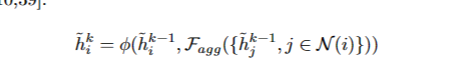
\includegraphics[width=10cm, height=2cm]{模型.png}
\end{figure}
其中包括了聚合函数 \(F_{\text{agg}}\),更新函数。模型通过聚集来自其邻居节点的信息以及它们之间的连接来对每个节点进行铺垫。

\subsection*{框架图}
\begin{figure}[htbp]
    \centering
    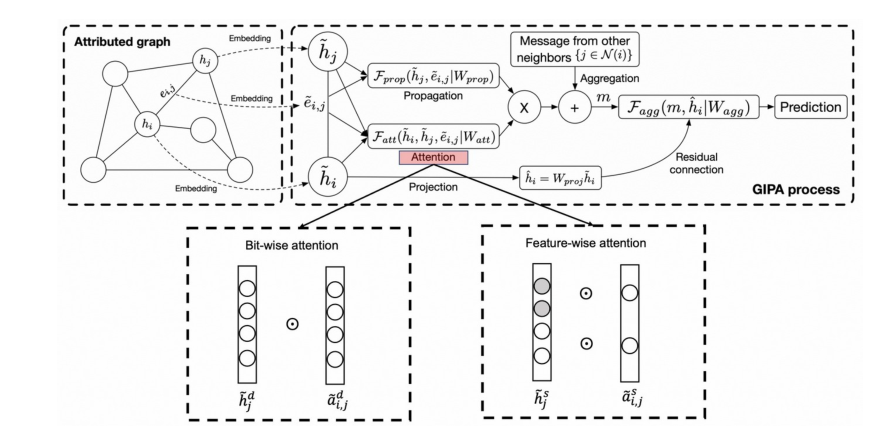
\includegraphics[width=11cm, height=8cm]{框架图.png}
\end{figure}
GIPA 的架构,由关注、传播和聚合模块(或过程)组成。红色阴影表示逐位模块和逐特征模块,它们通过更细粒度的选择性信息融合来提取与当前节点更相关的邻居信息。

\subsection*{工作流}
\textbf{嵌入层:}一个特征的稀疏嵌入需要更多的维度。对于每个类别功能,需要一键编码。例如,某个“类别特征”共有 \(K\) 个可能的类别,需要一个 \(K + 1\) 维向量来表示该特征。并将每个“统计特征”切割成 \(K\) 个类别(使用等频或等宽切割方法),然后进行 \(K + 1\) 维独热编码。
\clearpage % 强制图片开始新页面
\begin{figure}[htbp]
    \centering
    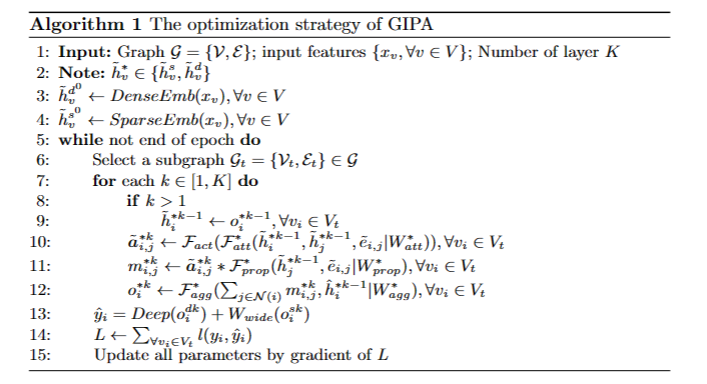
\includegraphics[width=9.5cm, height=8cm]{嵌入层优化.png}
\end{figure}

\section*{评价指标及其计算公式}
评估部分通过平均 ROC-AUC 分数来测量性能。
\begin{verbatim}
@torch.no_grad()
def evaluate(args, graph, model, labels, train_idx, val_idx, test_idx, criterion, evaluator):
    torch.cuda.empty_cache()
    model.eval()

    preds = torch.zeros(labels.shape).to(device)
    for _ in range(args.eval_times):
        for batch_nodes, subgraph in random_subgraph(args.eval_partition_num, graph, shuffle=False):
            subgraph = subgraph.to(device)
            pred = model(subgraph)
            preds[batch_nodes] += pred
    if args.eval_times > 1:
        preds /= args.eval_times

    train_loss = criterion(preds[train_idx], labels[train_idx].float()).item()
    val_loss = criterion(preds[val_idx], labels[val_idx].float()).item()
    test_loss = criterion(preds[test_idx], labels[test_idx].float()).item()
    train_score = evaluator(preds[train_idx], labels[train_idx])
    val_score = evaluator(preds[val_idx], labels[val_idx])
    test_score = evaluator(preds[test_idx], labels[test_idx])

    return train_score, val_score, test_score, train_loss, val_loss, test_loss, preds
\end{verbatim}
\texttt{evaluate} 函数用于评估模型性能。
\begin{itemize}
    \item \texttt{model.eval()} 将模型切换到评估模式,这会影响例如 \texttt{dropout} 的行为。
    \item 使用 \texttt{random\_subgraph} 函数生成随机子图进行评估。
    \item \texttt{args.eval\_times} 指定了对每个子图进行评估的次数,可以通过对多次评估取平均来减小随机性。
    \item 计算每个节点的预测值,并累加到 \texttt{preds} 中。
    \item 如果进行了多次评估,则将 \texttt{preds} 取平均。
    \item 使用预测值计算训练、验证和测试集的损失(\texttt{loss})和评估指标(\texttt{score})。
    \item 函数返回训练、验证和测试的损失和评估指标,以及所有节点的预测值 \texttt{preds}。
\end{itemize}

\section*{对比方法及其引用论文}
对比数据来自他们的论文或 OGB 排行榜。
\clearpage % 强制图片开始新页面
\begin{figure}[htbp]
    \centering
    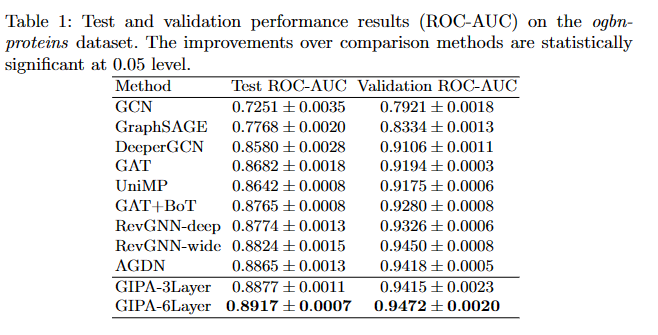
\includegraphics[width=9.5cm, height=8cm]{表现对比.png}
\end{figure}

\section*{结论}

\begin{verbatim}
./train_gipa.py --root ./ --train-partition-num 6 --eval-partition-num 2 --eval-times 1 --lr 0.01 --advanced-optimizer --n-epochs 1500 --n-heads 20 --n-layers 6 --dropout 0.4 --n-hidden 50 --input-drop 0.4 --edge-drop 0.1 --edge-agg-mode single_softmax --edge-att-act none --norm none --edge-emb-size 16 --gpu 0 --first-hidden 225 --use-sparse-fea --sparse-encoder log --n-deep-layers 6 --n-deep-hidden 200 --deep-drop-out 0.4 --deep-input-drop 0.1 --model gipa_deep_wide --log-file-name=run_default_wide_deep
Namespace(model='gipa_deep_wide', root='./', cpu=False, gpu=0, seed=0, n_runs=10, n_epochs=1500, eval_times=1, advanced_optimizer=True, train_partition_num=6, eval_partition_num=2, no_attn_dst=False, n_heads=20, norm='none', disable_fea_trans_norm=False, edge_att_act='none', edge_agg_mode='single_softmax', lr=0.01, n_layers=6, n_hidden=50, dropout=0.4, input_drop=0.4, edge_drop=0.1, eval_every=5, log_every=5, save_pred=False, log_file_name='run_default_wide_deep', first_hidden=225, edge_emb_size=16, wd=0, use_sparse_fea=True, sparse_encoder='log', input_norm=False, first_layer_norm=False, first_layer_act='relu', feature_drop=0.0, last_layer_drop=-1.0, n_deep_layers=6, n_deep_hidden=200, deep_drop_out=0.4, deep_input_drop=0.1)
Runned 10 times
Val scores: [0.9464610703119242, 0.945959865433455, 0.9422161149879379, 0.9481785285003014, 0.9472916867828222, 0.946567618075345, 0.9481510717785814, 0.9447355638872826, 0.9459294604587943, 0.9453477199621528]
Test scores: [0.8908229980036476, 0.8904088193170103, 0.8885491607462922, 0.8900243103672817, 0.8902722394523298, 0.8907890818798613, 0.8912160152904612, 0.8909373211380868, 0.8924123063424335, 0.8888346735752816]
Average val score: 0.9460838700178597 ± 0.0016689705092338104
Average test score: 0.8904266926112687 ± 0.001065859035608153
\end{verbatim}

\textbf{模型配置:}

\begin{verbatim}
模型类型: gipa_deep_wide
优化: 启用了高级优化器 (advanced_optimizer=True)。
架构:
  宽度部分: 模型有一个宽度部分,具有参数如 first_hidden、edge_emb_size 等。
  深度部分: 模型有一个深度部分,具有参数如 n_deep_layers、n_deep_hidden、deep_drop_out 等。
训练设置:
  学习率: 0.01 (lr=0.01)
  训练轮数: 1500 (n_epochs=1500)
  批标准化: 未应用标准化 (norm='none')。
  Dropout: 应用了各种不同的丢失率 (dropout, input_drop, edge_drop, deep_drop_out, deep_input_drop等)。
稀疏特征: 使用了稀疏特征 (use_sparse_fea=True),并使用了指定的稀疏编码器 (sparse_encoder='log')。
评估: 进行了多次评估 (eval_times=1),在指定的间隔 (eval_every=5)。
\end{verbatim}

\textbf{训练结果(共10次运行):}

\begin{verbatim}
验证分数: 每次运行的验证分数列表。
测试分数: 每次运行的测试分数列表。
平均验证分数: 在10次运行中,验证分数的平均值和标准差。
平均测试分数: 在10次运行中,测试分数的平均值和标准差。
\end{verbatim}

\textbf{解释:}

\begin{verbatim}
该模型在验证集上表现良好,平均验证分数约为 0.9461,标准差较低(± 0.0017)。
在测试集上的性能也是合理的,平均测试分数约为 0.8904,标准差较低(± 0.0011)。
所得到数据与论文吻合。
\end{verbatim}

\end{document}
